\subsection{Search}
After the EcoData team addressed the issues with storing semi-structured data, the next 
big problem to address was how to efficiently search through the data. The interface 
that was desired was one much like Google's search; a simple search box, with two
buttons. The interface needs to be extremely simple, but powerful, for it to be 
affective for non-technical users. 

\begin{figure}[h]
	\begin{center}
	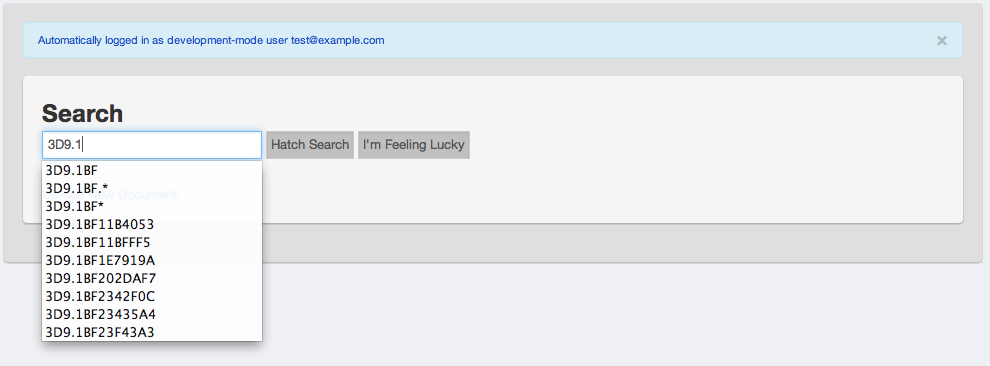
\includegraphics[width=120mm]{images/search_ss1}
	\caption{The search interface} 
	\label{search_ss1}
	\end{center}
\end{figure}

For example, when a user entered in a search like '3D9.1', it would be assumed that 
any data starting with '3D9.1' should be returned. Because Hatch assumes that
the user would want any data in the same row as the matching data, it returns
the entire row. 

For search, this leaves the possibility for a huge amount of string comparisons to find
all values that match. This would make search impractically slow. Luckily, CouchDB comes
to the rescue for us.


\subsubsection{Views}
CouchDB uses precompiled queries called \textbf{views}. Views take developer defined
query templates and apply them to every document that is created or updated in the 
database, when the document is saved. The result are precomipled lookout tables 
(actually heaps/binary trees), which make searches fast. 

Hatch basically creates a view like the following pseudocode:
\begin{lstlisting}
	for each document
		for each row
			for each column value in row
				emit(value, row)
\end{lstlisting}

\textbf{emit()} is a function that tells CouchDB how to make the search B-Tree. It 
takes two arguments; the key that the tree node will take, and the value that the 
node will return if the key matches the search. Hatch says 'every column value in a 
document is a key, and the return value is the data row it belongs to'. So if a search
matches a document value, the search results show the entire data row.

CouchDB makes Hatch's job easier by having internal methods for string matching. For
example, if a search for '3D9.1' is used with CouchDB startkey, CouchDB will return
any string starting with '3D9.1'. Hatch doesn't have to invent a query language to 
tell the database lots of parameters for matching values.

\begin{figure}[h]
	\begin{center}
	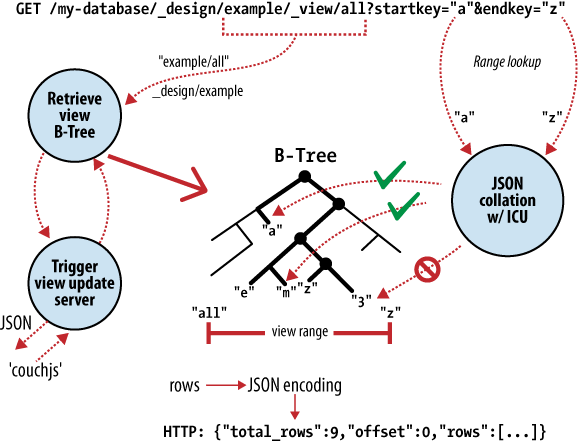
\includegraphics[width=120mm]{images/couchdb_b_tree}
	\caption{CoucbDB search through its internal binary tree.} 
	\label{couchdb_b_tree}
	\end{center}
\end{figure}

The other advantage to CouchDB is that it stores values in the B-Tree structure. For
string data types, this means that the database only within the '3D9.1' string range
in the tree. When the search sees a child node starting with '3D9.0', it instead picks
the child node staring with '3D9.1', and the entire '3D9.0' group is never searched 
through. 
